% Assignment 1 report: Analysis of SVD for Fine-Tuning LLMs
% Compile on Overleaf with XeLaTeX (Menu -> Compiler) for the Chinese name.
% pdfLaTeX also works: the name is then typeset with the CJKutf8 package.
\documentclass[10pt,a4paper]{article}

\usepackage[a4paper,margin=2cm]{geometry}
\usepackage{iftex}
\ifXeTeX
  \usepackage{xeCJK}
  \setCJKmainfont{Noto Serif CJK TC}
  \newcommand{\cjkname}[1]{#1}
\else
  \usepackage[utf8]{inputenc}
  \usepackage[T1]{fontenc}
  \usepackage{CJKutf8}
  \newcommand{\cjkname}[1]{\begin{CJK}{UTF8}{bkai}#1\end{CJK}}
\fi
\usepackage{amsmath,amssymb}
\usepackage{graphicx}
\usepackage{tabularx}
\usepackage{array}
\usepackage{enumitem}
\usepackage{caption}
\usepackage[hidelinks]{hyperref}

\setlength{\parindent}{0pt}
\setlength{\parskip}{3pt}
\setlist[itemize]{itemsep=1pt,topsep=2pt}
\newcolumntype{C}{>{\centering\arraybackslash}X}

\begin{document}

\begin{center}
  {\large\bfseries Assignment 1: Analysis of SVD for Fine-Tuning LLMs}\\[4pt]
  \cjkname{蕭至恆} (Student ID 413551034) \\
  GitHub: \url{https://github.com/CH-Joshua-Hsiao/NYCU-BigDataAnalytics/tree/main/HW1}
\end{center}
\textbf{Setup:} I fine-tuned Llama-3.2-1B with PiSSA on 25,000 MetaMathQA samples (1 epoch, learning rate
$2\times10^{-5}$, batch size 128, FP16, all 7 projection layers). I tested on 1,000 GSM8K and 1,000 MATH questions.
All runs used one RTX 3090 (24 GB) on my own computer, with micro-batch 4 and 32 accumulation steps. The SVD step
ran on the CPU.

% ------------------------------------------------------------------ Q1
\subsection*{Question 1: Accuracy of the original and fine-tuned models}
\begin{center}\small
\begin{tabularx}{\textwidth}{|l|C|C|C|C|}
  \hline
  \textbf{Accuracy} & \textbf{Original LLM} & \textbf{Fine-Tuned (RANK = 16)} & \textbf{Fine-Tuned (RANK = 64)} & \textbf{Fine-Tuned (RANK = 256)} \\
  \hline
  \textbf{GSM8K} & 3.4\% & 15.6\% & 20.7\% & 27.3\% \\ \hline
  \textbf{MATH}  & 0.1\% & 3.7\%  & 4.8\%  & 5.4\%  \\
  \hline
\end{tabularx}
\end{center}

\begin{itemize}
  \item \textbf{Original model.} The original model is very weak: 3.4\% on GSM8K and 0.1\% on MATH. It is a base
  model, not a chat model, so it does not really solve the question. In about half of the answers, it just repeats
  the same sentence again and again. Only 37 GSM8K answers and 41 MATH answers give a clear final answer (like ``The answer is:'',
  ``\#\#\#\#'' or \verb|\boxed{}|). For MATH, 959 answers have no answer that the parser can find. After
  fine-tuning on MetaMathQA, the model learns to solve step by step and to write the answer in the right format.
  So even rank 16 goes up to 15.6\% / 3.7\%.
  \item \textbf{Effect of rank.} When the rank is bigger, the accuracy is higher on both datasets: GSM8K
  15.6\% $\to$ 20.7\% $\to$ 27.3\%, and MATH 3.7\% $\to$ 4.8\% $\to$ 5.4\%. A bigger rank means more trainable
  parameters (0.9\% $\to$ 3.6\% $\to$ 14.6\% of the model). Also, in PiSSA, a bigger rank means the adapter starts
  from more of the main (principal) parts of the weight. So with the same learning rate and one epoch, the model
  can change more. The final training loss also goes down (0.455 $\to$ 0.414 $\to$ 0.375).
  \item \textbf{Format or reasoning?} I also checked if the model only learns the answer format. The table below
  shows how many answers have a clear final answer, and the accuracy of these answers. On GSM8K, the number is
  almost the same after rank 16 (951, 957, 954), so the format is already learned. But the accuracy still goes up
  (16.4\% $\to$ 21.6\% $\to$ 28.6\%). This means a bigger rank really helps the reasoning, not only the format. On
  MATH, both become better: more clear answers (452 $\to$ 547) and higher accuracy (8.2\% $\to$ 9.9\%). However,
  the reasoning is still not good. Many answers have a nice format but wrong calculation.
\end{itemize}

\begin{center}\small
\begin{tabularx}{\textwidth}{|p{3.6cm}|C|C|C|C|}
  \hline
  \textbf{Clear final answers (accuracy of them)} & \textbf{Original LLM} & \textbf{Fine-Tuned (RANK = 16)} & \textbf{Fine-Tuned (RANK = 64)} & \textbf{Fine-Tuned (RANK = 256)} \\
  \hline
  \textbf{GSM8K} & 37 (13.5\%) & 951 (16.4\%) & 957 (21.6\%) & 954 (28.6\%) \\ \hline
  \textbf{MATH}  & 41 (2.4\%)  & 452 (8.2\%)  & 523 (9.2\%)  & 547 (9.9\%)  \\
  \hline
\end{tabularx}
\end{center}

\begin{itemize}
  \item \textbf{GSM8K vs.\ MATH.} GSM8K improves much more than MATH (+11.7 points vs.\ +1.7 points from rank 16
  to 256). GSM8K questions are simple word problems, and they are similar to the MetaMathQA training data. Its
  accuracy is still going up at rank 256. MATH questions are much harder. They need more math knowledge and answers
  in LaTeX form (fractions, square roots, intervals). A 1B model cannot learn this from 25k samples in one epoch.
  About 45\% of MATH answers still have no answer that the parser can find, so MATH improves only a little.
\end{itemize}

% ------------------------------------------------------------------ Q2
\subsection*{Question 2: Training time}
\begin{center}\small
\begin{tabularx}{0.9\textwidth}{|l|C|C|C|}
  \hline
  & \textbf{Fine-Tuned (RANK = 16)} & \textbf{Fine-Tuned (RANK = 64)} & \textbf{Fine-Tuned (RANK = 256)} \\
  \hline
  \textbf{Training Time (min.)} & 36.0   & 38.8   & 64.0    \\ \hline
  \textbf{Trainable Parameters} & 11.3 M & 45.1 M & 180.4 M \\
  \hline
\end{tabularx}
\end{center}

\begin{itemize}
  \item \textbf{Trend.} From rank 16 to 64, the trainable parameters become 4 times more, but the training time
  only increases by 2.7 minutes (+8\%). From rank 16 to 256, the parameters become 16 times more, and the time
  becomes 64.0 minutes (+78\%). So the training time increases with the rank, but much slower than the number of
  parameters.
  \item \textbf{Reason.} Most of the training time is used to run the big frozen model (1.2B parameters) forward
  and backward. This part does not depend on the rank. The adapter only adds two small matrix multiplications. Their
  cost is $r(d+k)$, while the original weight costs $dk$. For a $2048\times2048$ layer, this is only about 1.6\%
  more at $r=16$, but about 25\% more at $r=256$. The adapter also needs its own weight gradients. In addition,
  rank 256 has 180M trainable parameters, and AdamW keeps extra states for each of them, so the optimizer step is
  also slower. That is why the time is almost the same for small ranks, and only becomes clearly longer at rank 256.
  The SVD step at the beginning (about 100 seconds on the CPU) is not included. It takes the same time for all
  ranks, because the code always computes the full SVD.
\end{itemize}

% ------------------------------------------------------------------ Q3
\subsection*{Question 3: Fine-tuning different singular-value ranges (rank 16)}
\begin{center}
  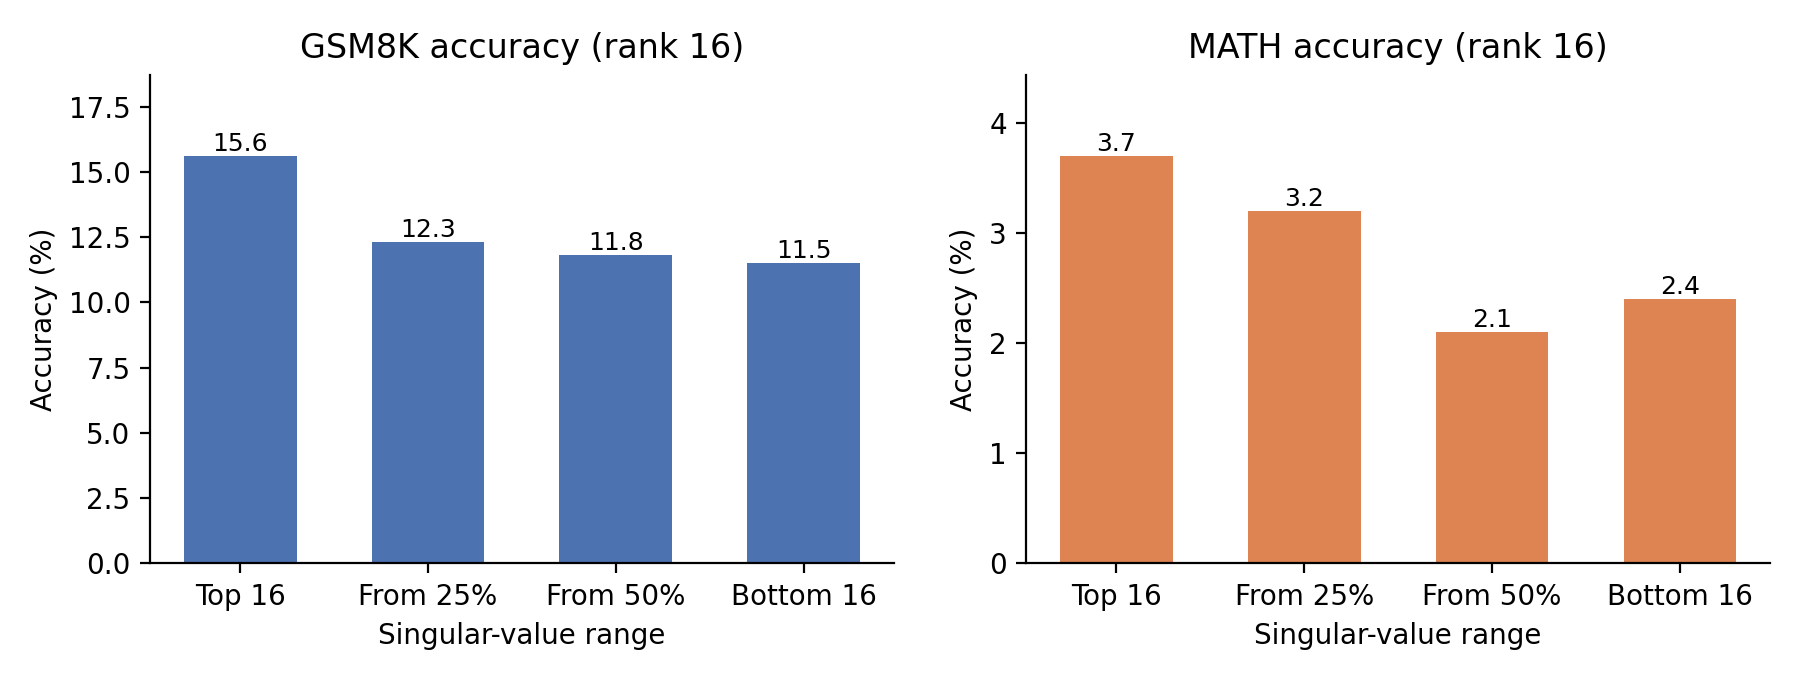
\includegraphics[width=0.85\textwidth]{figures/q3_components.png}\\[2pt]
  \small
  \begin{tabularx}{0.85\textwidth}{|l|C|C|C|C|}
    \hline
    \textbf{Range} & \textbf{Top 16} & \textbf{From 25\%} & \textbf{From 50\%} & \textbf{Bottom 16} \\
    \hline
    \textbf{GSM8K} & 15.6\% & 12.3\% & 11.8\% & 11.5\% \\ \hline
    \textbf{MATH}  & 3.7\%  & 3.2\%  & 2.1\%  & 2.4\%  \\
    \hline
  \end{tabularx}
\end{center}

\begin{itemize}
  \item \textbf{Trend.} The top 16 singular values give the best result on both datasets (15.6\% on GSM8K, 3.7\%
  on MATH). When we use smaller singular values, the accuracy becomes lower: 12.3\% / 11.8\% / 11.5\% on GSM8K and
  3.2\% / 2.1\% / 2.4\% on MATH (from 25\%, from 50\%, bottom). The training loss has the same order (average of
  the last 10 steps: 0.419, 0.462, 0.467, 0.476). The three non-top ranges are very close, within about 1 point.
  With only 1,000 test questions, the random error is about 1 point on GSM8K and 0.5 point on MATH. So I think
  these three are about the same, and only the top 16 is clearly better. The top 16 is better in both format and
  reasoning: on GSM8K it gives more clear answers (951 vs.\ 859--904), and these answers are more accurate
  (16.4\% vs.\ 12.8--13.5\%).
  \item \textbf{Why the top 16 is the best.} In PiSSA, the adapter starts as $A = U_r\sqrt{S_r}$ and
  $B = \sqrt{S_r}\,V_r^{\top}$. So the model can only change the part of the weight that we choose. The top
  singular values have most of the energy. From Q4, the top 16 have 15--35\% of the energy of q\_proj, but 16
  values at the 25\% or 50\% position have only about 0.1--0.7\%. These top directions are the ones the layer
  really uses, so changing them has the biggest effect. Also, $A$ and $B$ are bigger at the start, so their
  gradients are bigger ($\partial L/\partial A \propto B$, $\partial L/\partial B \propto A$), and the model learns
  faster. The middle and bottom directions are very small and the original model almost does not use them, so
  changing them helps less.
  \item \textbf{Why the other ranges still work.} Even the bottom 16 (singular values close to 0) is much better
  than the original model (3.4\% $\to$ 11.5\% on GSM8K). One reason is AdamW: it scales each update by the gradient
  size, so even very small $A$ and $B$ still move about one learning rate per step. Also, 16 dimensions are enough to
  learn the answer format and some simple reasoning. Using the top 16 gives about 3--4 more points on GSM8K. This
  matches the PiSSA paper, which says that training the principal parts learns faster and works better than training
  the small parts.
\end{itemize}

% ------------------------------------------------------------------ Q4
\subsection*{Question 4: SVD of q\_proj in the original model (layers 0, 7, 15)}
\begin{center}\small
\begin{tabularx}{0.9\textwidth}{|p{5.2cm}|C|C|C|}
  \hline
  & \textbf{Layer 0} & \textbf{Layer 7} & \textbf{Layer 15} \\
  \hline
  \textbf{Minimum Target Rank for query projection weights ($\geq$ 50\% energy)} & \textbf{62} & \textbf{120} & \textbf{84} \\ \hline
  $\sigma_1$ / $\sigma_{16}$                        & 31.4 / 5.7 & 10.3 / 4.2 & 12.9 / 4.7 \\ \hline
  Energy in top 16 / top 200                        & 34.8\% / 71.2\% & 15.4\% / 63.5\% & 21.0\% / 68.8\% \\
  \hline
\end{tabularx}
\end{center}

\begin{figure}[h]
  \centering
  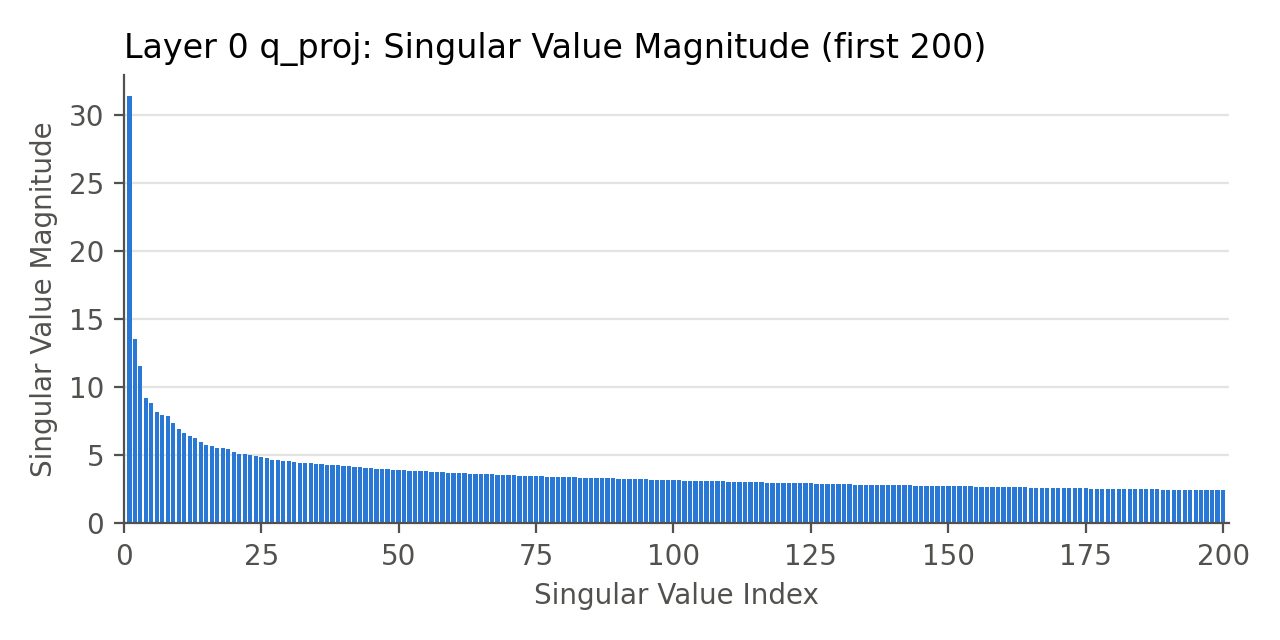
\includegraphics[width=0.49\textwidth]{figures/layer0_singular_values.png}\hfill
  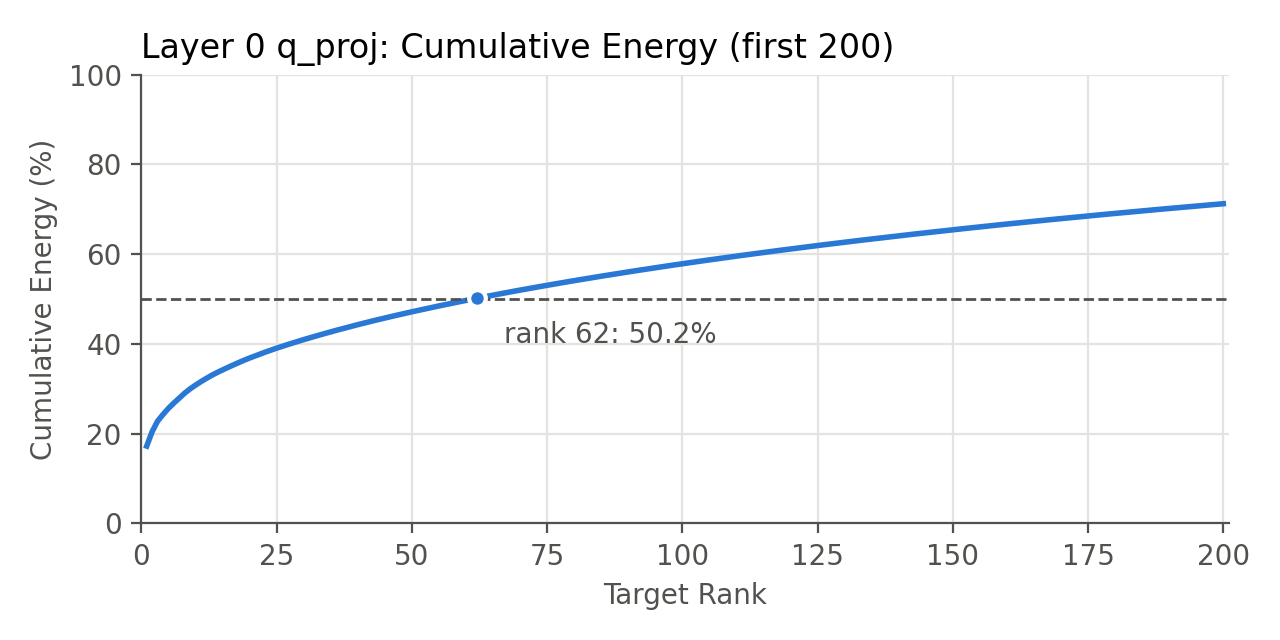
\includegraphics[width=0.49\textwidth]{figures/layer0_cumulative_energy.png}\\[2pt]
  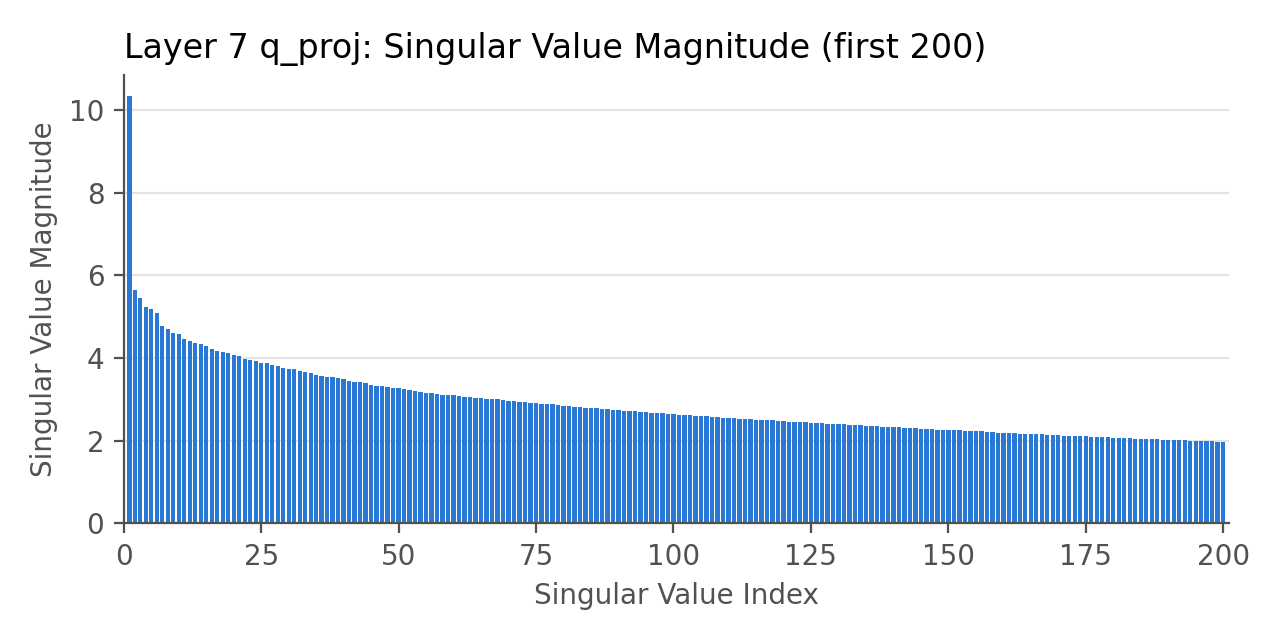
\includegraphics[width=0.49\textwidth]{figures/layer7_singular_values.png}\hfill
  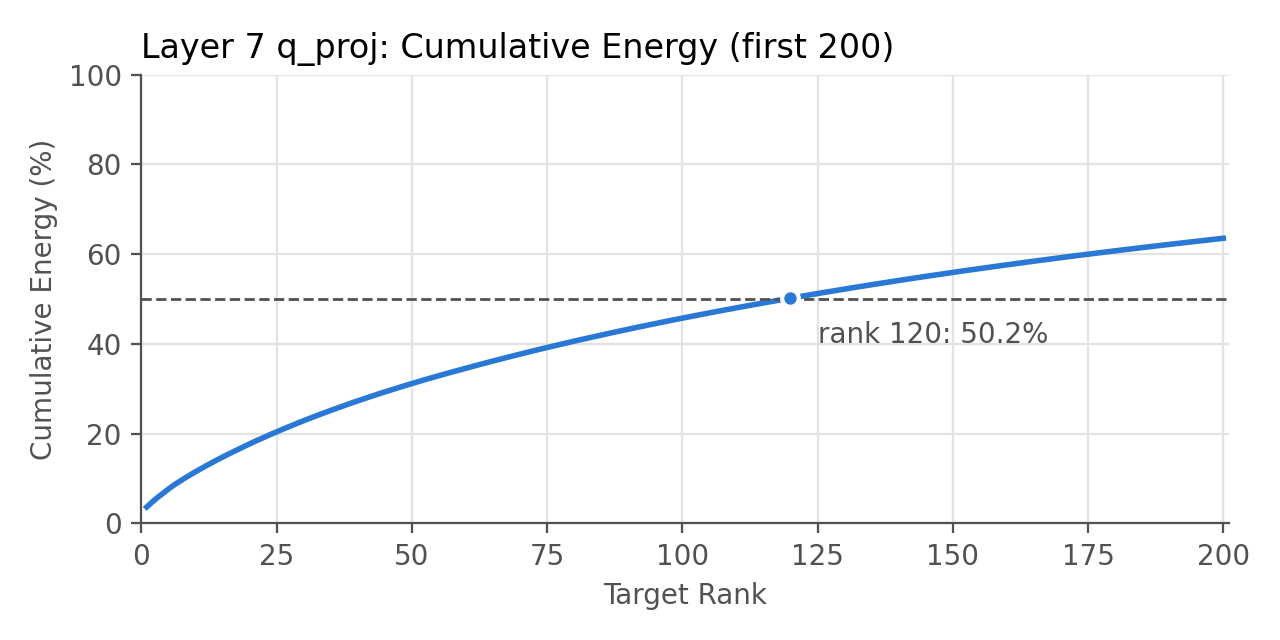
\includegraphics[width=0.49\textwidth]{figures/layer7_cumulative_energy.png}\\[2pt]
  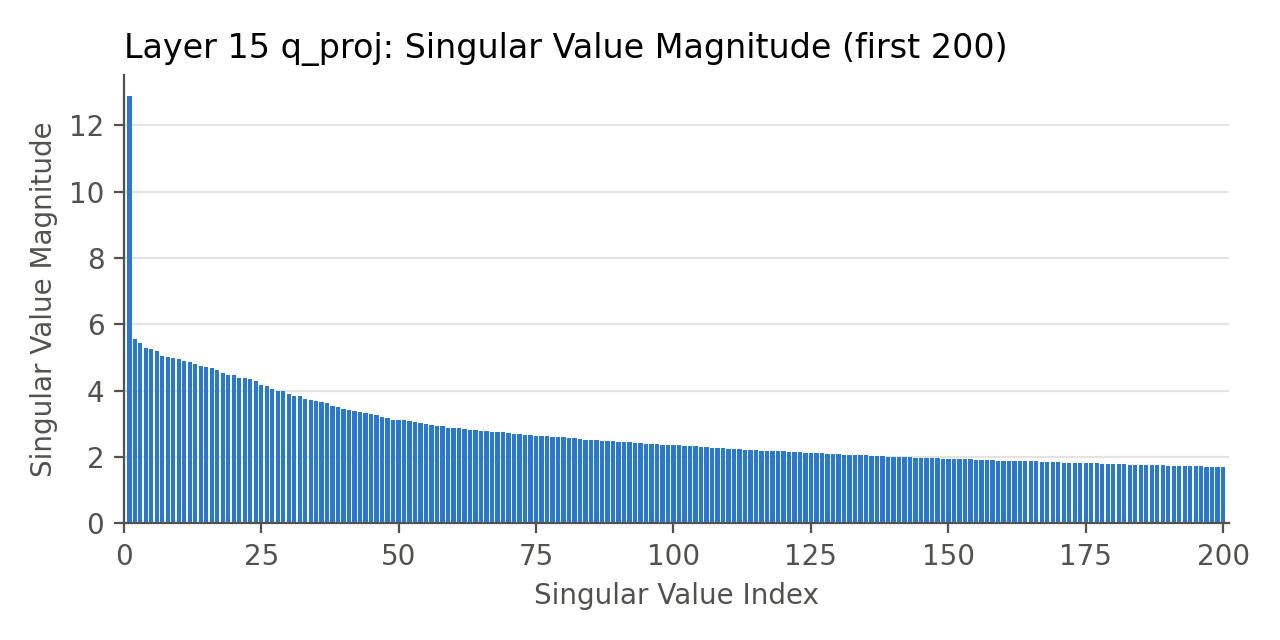
\includegraphics[width=0.49\textwidth]{figures/layer15_singular_values.png}\hfill
  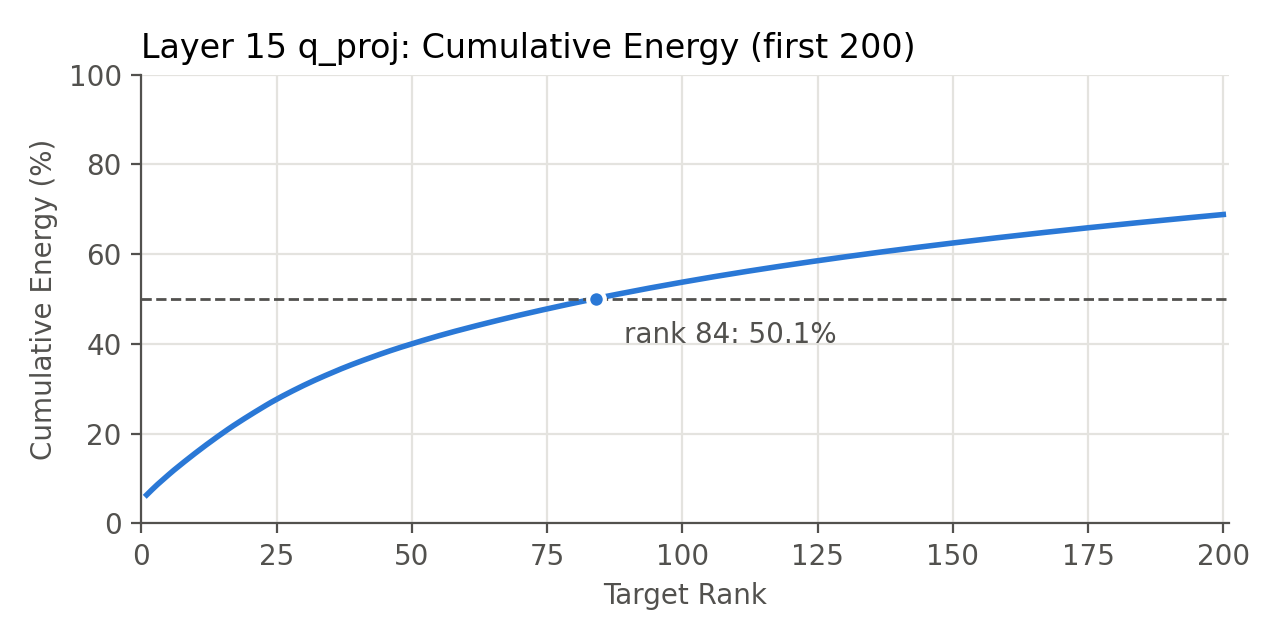
\includegraphics[width=0.49\textwidth]{figures/layer15_cumulative_energy.png}
  \caption*{Left: singular value magnitude (bar chart). Right: cumulative energy (line chart).
  Only the first 200 of 2,048 singular values are shown. Energy $=\sum_{i\le r}\sigma_i^2 / \sum_i \sigma_i^2$.
  The dashed line is 50\%.}
\end{figure}

\begin{itemize}
  \item \textbf{Shape.} All three layers have a similar shape. There are a few large singular values at the
  beginning ($\sigma_1$ is about 2.5--5.5 times $\sigma_{16}$), and then a long and almost flat tail. To keep 50\% of the
  energy, we only need 62--120 of the 2,048 values (3--6\% of the full rank). But even the first 200 values only
  keep 63--71\% of the energy. So the weight is not really low-rank. The rest of the energy is spread over many
  small values.
  \item \textbf{Differences between layers.} Layer 0 is the most concentrated. $\sigma_1 = 31.4$ is much bigger
  than the others, and the top 16 have 34.8\% of the energy. Layer 7 is the most spread out (only 15.4\% in the
  top 16, and it needs rank 120). Layer 15 is in the middle (rank 84). My guess is that layer 0 works directly on
  the token embeddings, so a few main directions carry most of the information. Middle layers mix many different
  features, so they use more directions. The last layers focus more again on predicting the next token.
  \item \textbf{What this means.} If we use the same rank for every layer, each layer keeps a very different amount
  of energy. For example, rank 16 keeps about 35\% of the energy in layer 0, but only 15\% in layer 7. This
  supports the idea of PiSSA (training the principal part). It also suggests that giving different ranks to
  different layers may use the parameters better.
\end{itemize}

\end{document}
